\documentclass[border=10pt,varwidth=30cm]{standalone}
\usepackage{graphicx}
\usepackage[export]{adjustbox} % Needed for letters to align with top
\usepackage{tikz}
\usepackage{multirow}

\begin{document}
\begin{figure}
\begin{tabular}[t]{cc}
  \multicolumn{2}{c}{\textit{A. Americanus} Population Structure} \\
\multirow{2}{0.1\textwidth}{\includegraphics[valign=t,angle=-90,origin=c,width=0.1\textwidth]{../structure/plots/americanus-minSamples99-mac3-popmap3-K-3.pdf}}
& \includegraphics[valign=t,width=0.4\textwidth]{../maps/out/structure-americanus-minSamples99-mac3-popmap3-K-3.pdf} \\
& \includegraphics[valign=t,width=0.2\textwidth]{../pca/out-plots/americanus-minSamples99-mac3-popmap3-pca.pdf} \\
\end{tabular}
\end{figure}
\end{document}

% \begin{document}
% \begin{figure}
% \begin{tabular}[t]{c}
%   \textit{A. Americanus} Population Structure \\
%   \includegraphics[valign=t,width=0.5\textwidth]{../structure/plots/americanus-minSamples99-mac3-popmap3-K-3.pdf} \\
%   \includegraphics[valign=t,width=0.5\textwidth]{../maps/out/structure-americanus-minSamples99-mac3-popmap3-K-3.pdf} \\
%   \includegraphics[valign=t,width=0.3\textwidth]{../pca/out-plots/americanus-minSamples99-mac3-popmap3-pca.pdf} \\
% \end{tabular}
% \end{figure}
% \end{document}


% \begin{document}
% \begin{figure}
% \noindent
% \setlength\tabcolsep{1.4pt}
% \begin{tabular}[t]{cccc}

%   % Row 1
%   {\textbf{\huge (A)}} & 
%   \multicolumn{3}{c}{\includegraphics[valign=t,width=0.9\textwidth]{
%       ../structure/plots/hybrid-zone-minSamples95-mac3-popmap2-K-2.pdf}} \\[3.55cm]

%   % Row 2
%   {\textbf{\huge (B)}} &  
%   \includegraphics[valign=t,width=0.41\textwidth]{
%       ../pca/out-plots/hybrid-zone-minSamples95-mac3-popmap2-pca.pdf} &
%   {\textbf{\huge (C)}} &
%   \includegraphics[valign=t,width=0.41\textwidth]{
%       ../pca/out-plots/hybrid-zone-minSamples95-mac3-popmap2-admx-coeff.pdf} \\[12.6cm]

%   % Row 3 
%   {\textbf{\huge (D)}} & 
%   \multicolumn{3}{c}{\includegraphics[valign=t,width=0.9\textwidth]{
%       ../maps/out/structure-hybrid-zone-minSamples95-mac3-popmap2-K-2.pdf}} \\

%   \begin{tikzpicture}[remember picture,overlay]
%     % \node[xshift=6.5cm,yshift=-4.8mm,anchor=north west] at (current page.north west){
%     % 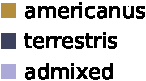
\includegraphics[width=30mm]{legend.pdf}};
%     \node[anchor=south east, yshift=3mm, xshift=27.5cm]{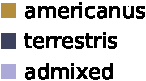
\includegraphics[width=30mm]{legend.pdf}};
%   \end{tikzpicture}

% \end{tabular}
% \end{figure}
% \end{document}